\documentclass{report}
\usepackage{graphicx}
\usepackage[width = 150mm, left=1in, right=1in, top=1.5in, bottom=1.5in]{geometry}
\usepackage{amsmath}
\usepackage{amsfonts}
\setlength{\parindent}{0pt}

\title{CT Report}
\author{Yuzhou Chen}
\date{\today}

\begin{document}
\maketitle
%page 1
\section[short]{PART 1}

The maximun angle of single projection could be calculated implimenting the following inequality:
\[
    \Delta \theta \leq \frac{2}{N_{\text{samples}}} = \frac{1}{96}
\]
Then the approximate number of projections could be gained: 
\[
    N_\theta = N_{\text{proj}} \geq \frac{\theta_{\text{max}}-\theta_{\text{max}}}{\Delta \theta} = 96 \pi \approx 301.592
\]
Since part 9. and part 10. request $ N_{\text{proj}}$ to be a multiple of $4$, we can Impliment the following value:
\[
    N_\theta = 304
\]

Thus 236 projections would be enough to fully sample the object for a final
image of size 192 by 192.
\begin{figure}[hb]
    \centering
    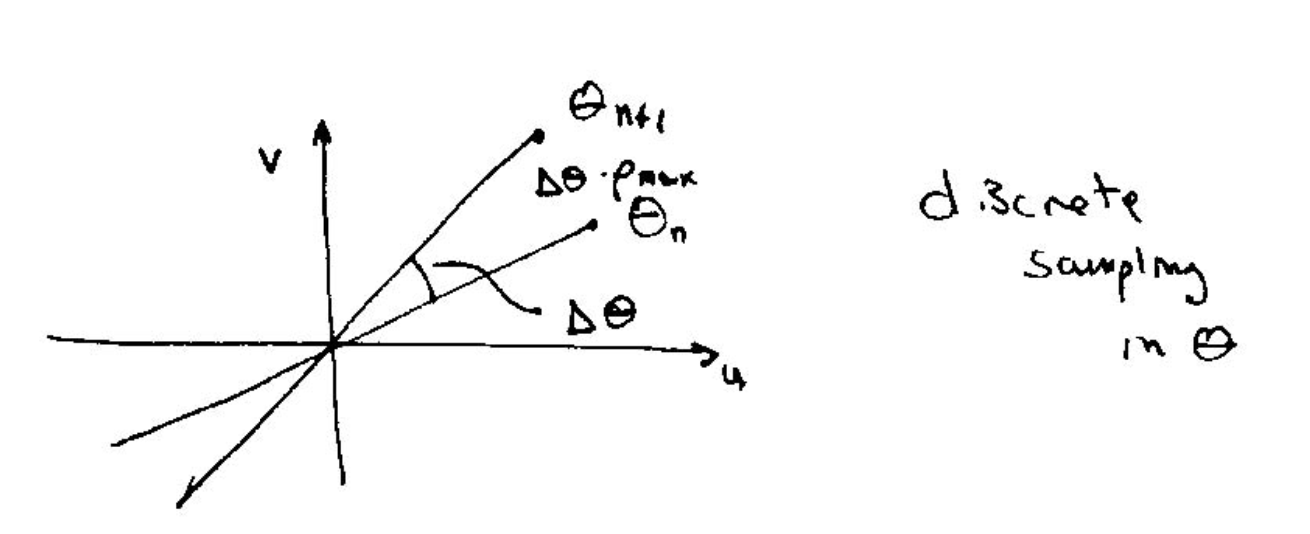
\includegraphics[width=1\textwidth]{1.png}
    \caption{Sampling in $\theta$.}
\end{figure}  

\newpage
%page 2
\section[short]{PART 2}
The sinogram could be implemented by the following equation, where $R_0 = 192mm$:
\begin{align*}
g_{\theta}(R) = 
\begin{cases} 
2\text{amplitude}\sqrt{R_0^2 - \left( R - x_0\cos\theta - y_0\sin\theta \right)^2},
& \text{if } \left| R - x_0\cos\theta - y_0\sin\theta \right| < R_0 \\
0, & \text{else}
\end{cases}
\end{align*}

By contrast to the CT-note, we can guess the image is a small cirle located at 
$x = -53mm$ and a larger circle located at $x = 30mm$, represented as two bright 
hyperbolic curves. And for the y axis, the small circle looks symmetrical which means $y = 0$. 
But for the larger circle, it is hard to guess the location.\vspace{\baselineskip}

And the other colored part through the whole image from $x = -75mm$ to $x = -75mm$
is the largest circle which located at the origin of the axis, which shown a symmetrical
shape as a rectangle.\vspace{\baselineskip}

In summary, three circle will be represented in the image in the next task.

\begin{figure}[hb]
    \centering
    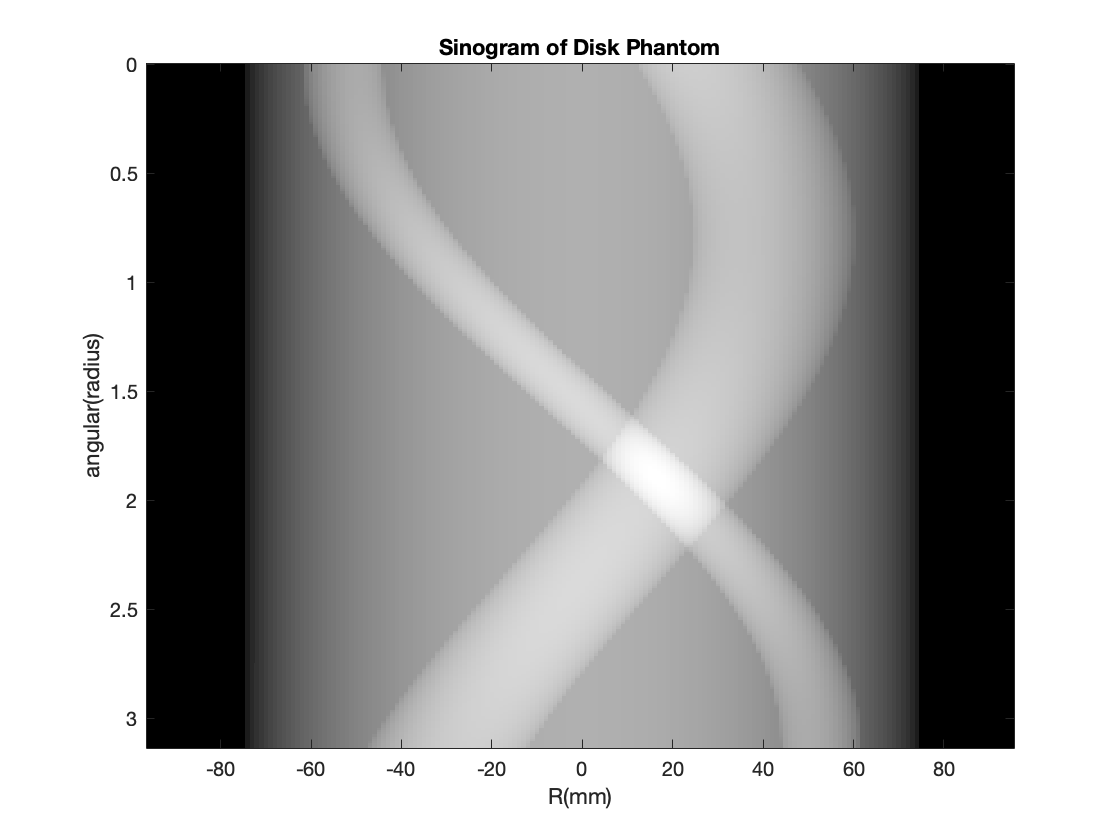
\includegraphics[width=1\textwidth]{2.png}
    \caption{Sinogram.}
\end{figure}  
\newpage
%page 3
\section[short]{PART 3}
Impliment the followng equation to finish the rotation of projection at each angular:
\[
b_{\theta}(x, y) = \int_{-\infty}^{\infty} g_{\theta}(R)\delta(x\cos\theta + y\sin\theta - R)dR
\]
Then we need to sum all the projections together by implimenting the following equation:
\[
f_b(x,y) = \int_{0}^{\pi} b_{\theta}(x, y)d\theta
\]
Then the plotting of final image could be shown in the $Figure.3$.The result of
such a simple backprojection is typically very blurry and has a starburst artifact
due to the high-intensity contributions along the straight paths of the X-rays.
This is visible in the second image you provided, where the blurry appearance and
overlapping regions of brightness reflect the basic nature of the backprojection
without any filtering to refine the result.

\begin{figure}[hb]
    \centering
    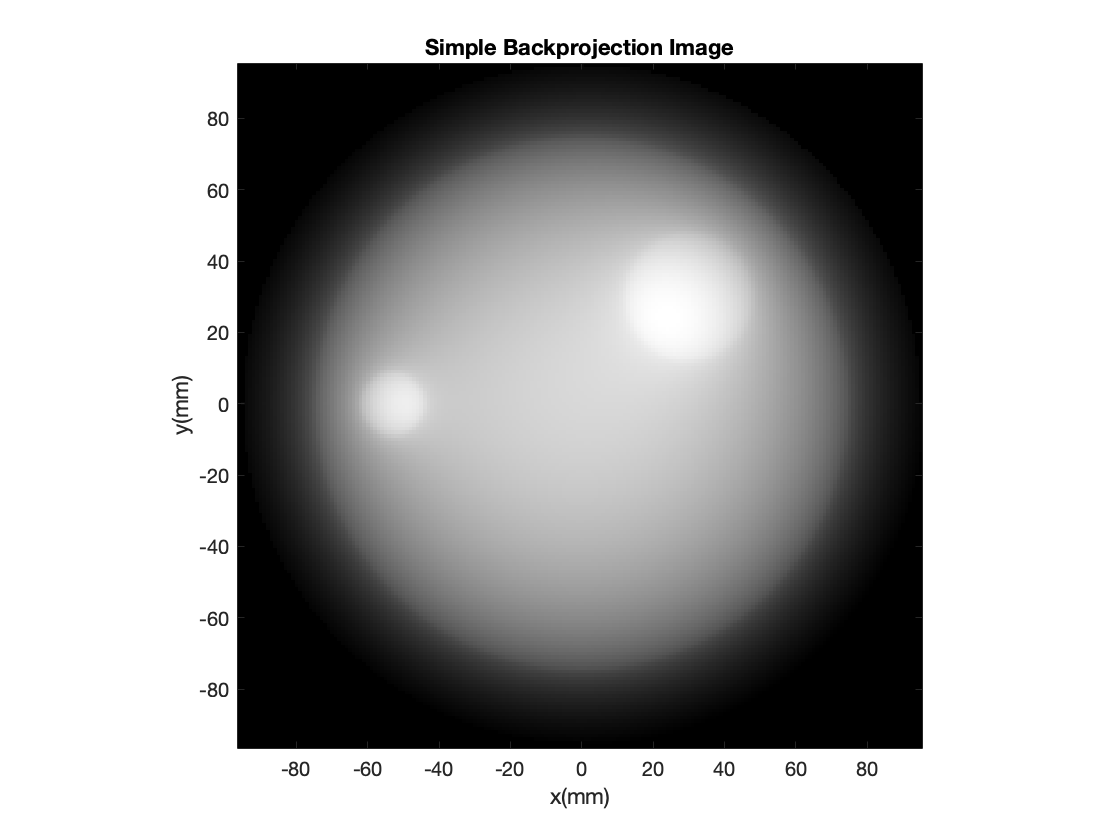
\includegraphics[width=1\textwidth]{3.png}
    \caption{Backprojection Image.}
\end{figure}  
\newpage

%page 4
\section[short]{PART 4}
To start the filtering, we can implement the "ramp" filter, which is also a 
high-pass filter by using the following equation:
\[
g'_{\theta}(R) = \mathcal{F}^{-1}\left\{ |\rho| \mathcal{F}_{1D} \{ g_{\theta}(R) \} \right\}
\]
From the plot, we can find out that the sharp edges in the filtered projection 
correspond to the boundaries of the object being imaged.The clear difference 
between the unfiltered and filtered projections is evident in the steepness and 
height of the graphs; the filtered projection has much steeper sides and a flat top,
which indicates that the filter has enhanced the high-frequency components corresponding
to the edges of the disk.
\begin{figure}[hb]
    \centering
    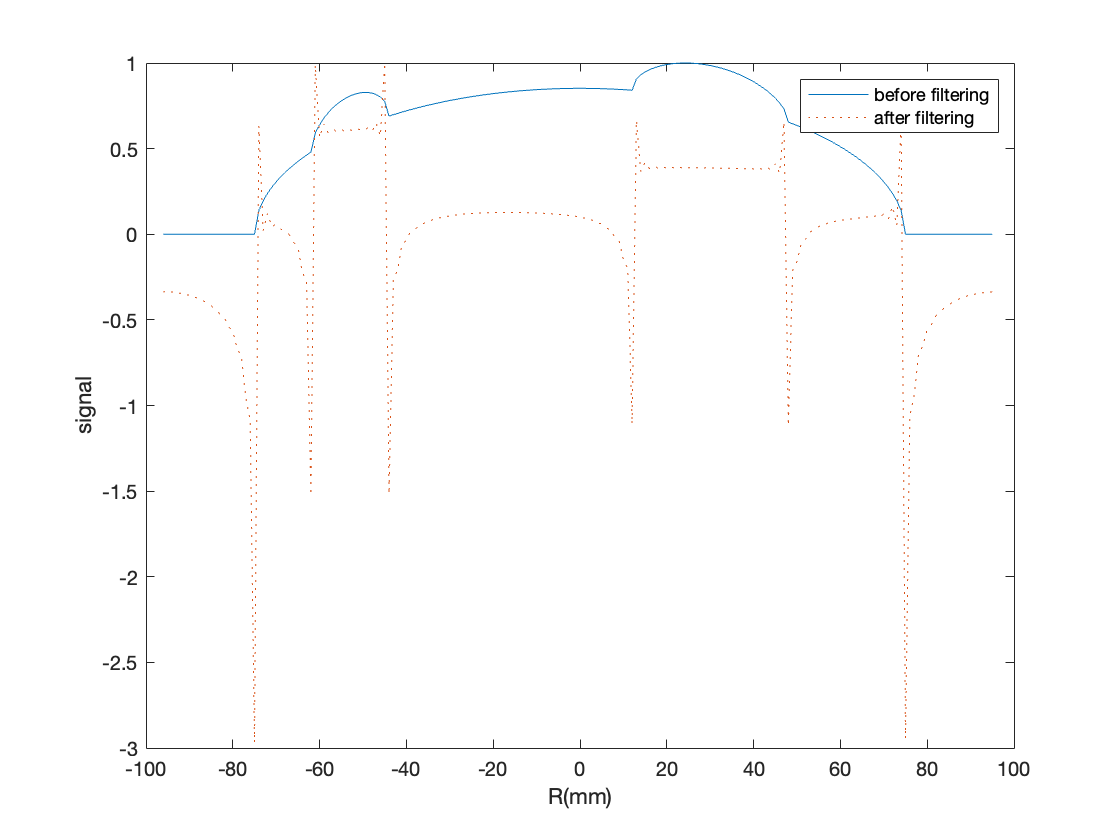
\includegraphics[width=1\textwidth]{4.png}
    \caption{Campared defference before filtered and after filtering.}
\end{figure}
\newpage  
%page 5
\section[short]{PART 5}
The filtering process enhances the high-frequency components associated with 
edges and reduces low-frequency components associated with smooth regions, leading 
to a clearer and more accurate reconstruction.\vspace{\baselineskip}

And from the reconstruction, here are some different kinds of artifact could be
found in the image:\vspace{\baselineskip}

1. \textbf{Streak Artifacts}: There may be some faint streaks emanating from the bright areas.
These are less pronounced than in an unfiltered image but can still occur if the
filter does not fully compensate for all the high-frequency loss during backprojection.\\
2. \textbf{Noise}: There's some level of graininess or noise in the image.\\
3. \textbf{Beam Hardening Artifacts}: These would manifest as dark bands or areas
that seem less dense than expected.

\begin{figure}[hb]
    \centering
    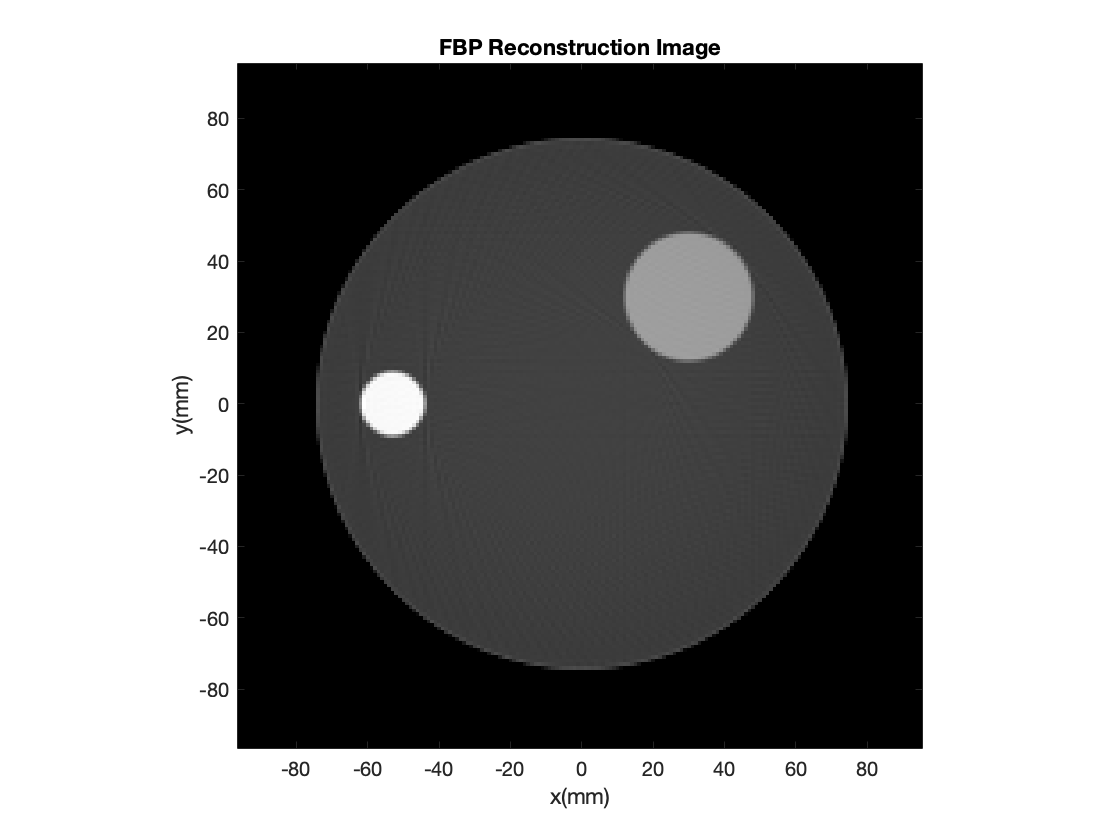
\includegraphics[width=1\textwidth]{5.png}
    \caption{FBP method.}
\end{figure}
\newpage 
%page 6
\section[short]{PART 6}
Firstly, take 1D-Fourier transform, which could be done by $ft$ function in $MATLAB$:
\begin{align*}
\mathcal{F}_{1D}\{g_{\theta}(R)\} = G_{\theta}(\rho) = F(\theta,\rho)
\end{align*}
Then, transfer the scale of image from polar to rectangular coordinates by using 
$griddat$ function:
\begin{align*}
    F(\theta,\rho) \Rightarrow \hat{F}(u, v)
\end{align*}
From the plot, we can notice there are different kinds of artifacts and the image
also looks blur with the strip-shape noise which needed further processing.\vspace{\baselineskip}

The following artifacts could be seen:

1. \textbf{Streak Artifacts}\\
2. \textbf{Noise}\\
3. \textbf{Unknow Artifact}: Since we are using $griddat$ function, there are artifacts generated because of the
repeated sampling in the origrin.\\
4. \textbf{Gibbs Phenomenon}: There might be ripples or oscillations near the edges of objects,
typically occurring near sharp transitions or boundaries in the image. This is due to the truncation of the Fourier series.
\begin{figure}[hb]
    \centering
    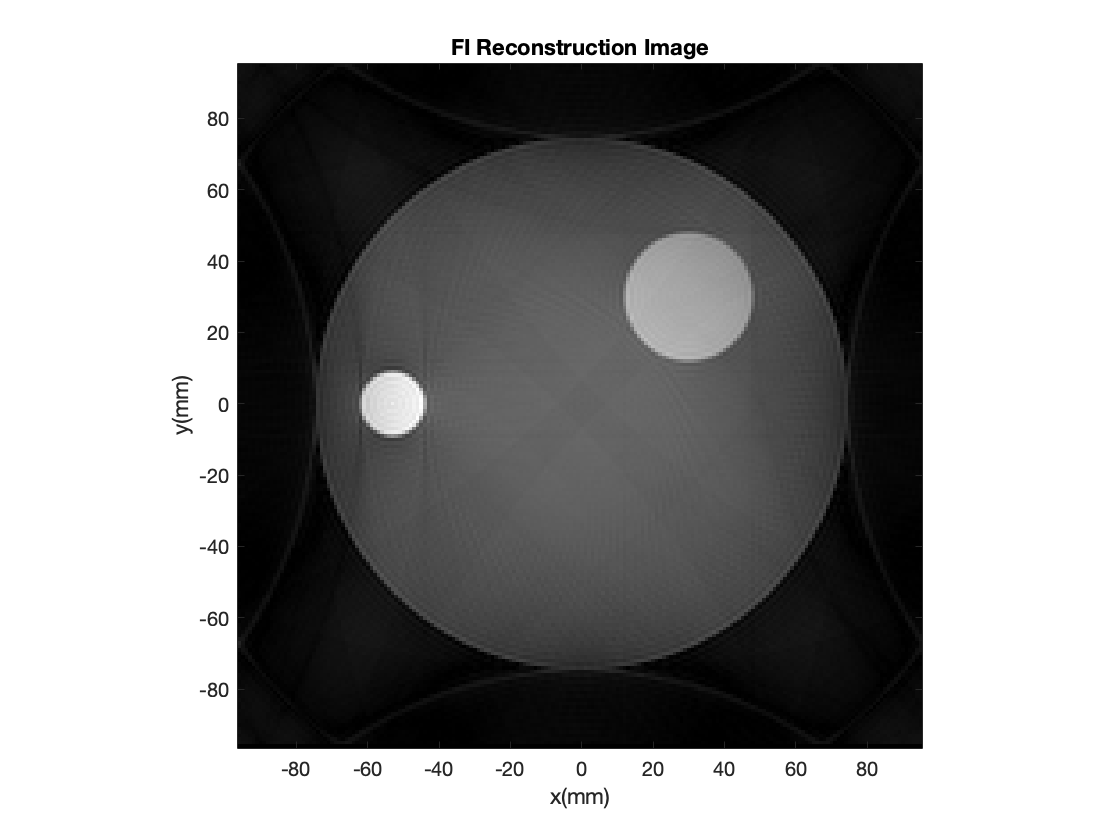
\includegraphics[width=0.75\textwidth]{6.png}
    \caption{FI Method}
\end{figure}
\newpage 
%page 7
\section[short]{PART 7}
By contrast to the FI reconstruction without zero pad, here is some difference:\\

1. \textbf{Noise}: The ZP image seems smoother with less visible noise, which might be due to the 
interpolation effect of the zero padding that can lead to a smoothing of the image.\\

2. \textbf{Artifacts}: All the tyoes of artifacts was reduced after zero padding\\

3. \textbf{Background}: The zero padding seems to improve the uniformity and consistency of the background, 
making the objects in the image stand out more clearly against the background.\\

In summary, zero padding effectively increases the number of samples in the Fourier domain, 
leading to a finer grid upon inverse transformation. This does not add new information 
but interpolates existing data, which can improve the image quality by reducing 
artifacts and enhancing resolution. The improvement in image quality from part 6
to part 7 is consistent with the expected effects of zero padding in Fourier-based
image reconstruction methods.
\begin{figure}[hb]
    \centering
    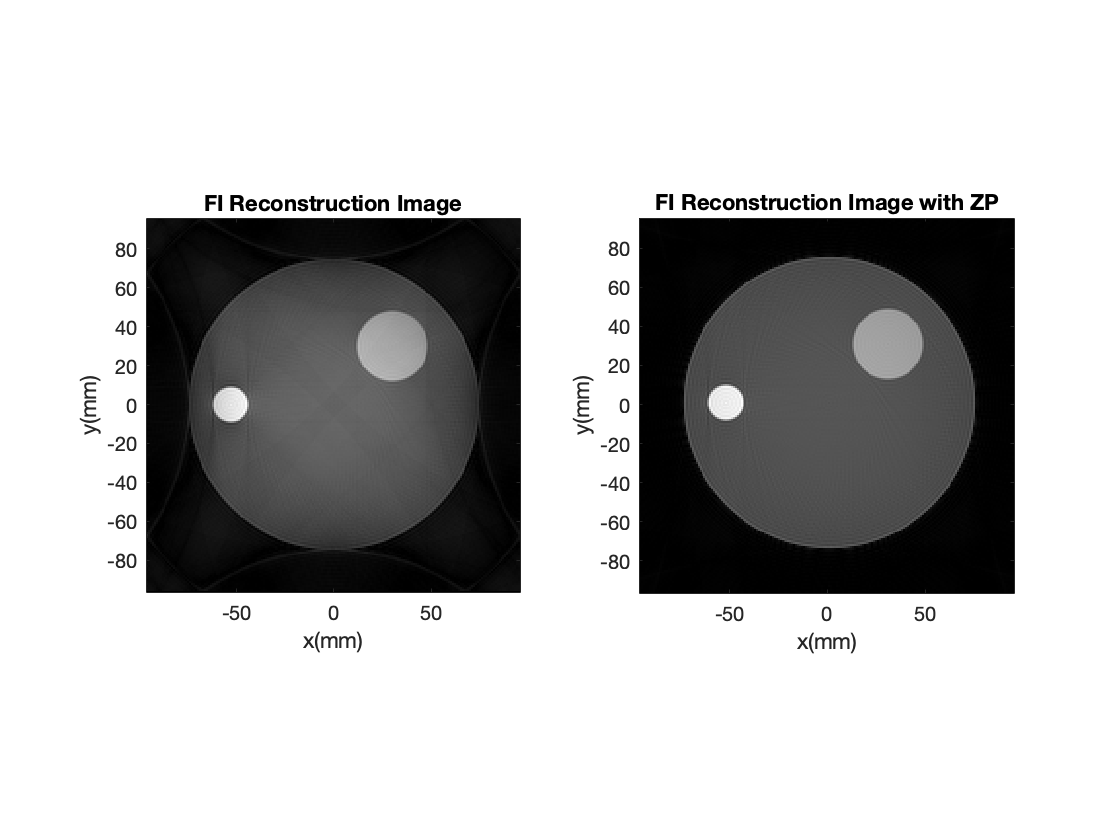
\includegraphics[width=0.75\textwidth]{7.png}
    \caption{FI method with zero pad.}
\end{figure}
\newpage 
%page 8
\section[short]{PART 8}
1. \textbf{FBP Profile (Solid Blue Line)}: This profile appears to have the highest overall 
intensity and shows a clear distinction between the high-intensity areas (presumably
corresponding to the more attenuating regions within the phantom) and the background. 
However, there is some fluctuation in intensity near the edges, which could be 
indicative of the Gibbs phenomenon or other reconstruction artifacts like noise.\\

2.\textbf{FI Profile (Dashed Orange Line)}: The FI profile without zero padding shows significantly
lower intensity, suggesting that the image might be under-scaled compared to the FBP image. 
The peaks are also less sharp, which could be due to a smoothing effect inherent
to the interpolation process.\\

3.\textbf{FI ZP Profile (Yellow Line)}: The profile of the FI image with zero padding seems 
to have a slightly higher intensity than the FI without ZP and is smoother, indicating 
that zero padding may help in reducing noise and improving the uniformity of the 
reconstructed image. However, there is a noticeable peak on the right side that 
does not align with the FBP profile, which might suggest an artifact introduced 
by the zero padding or the interpolation process.


\begin{figure}[hb]
    \centering
    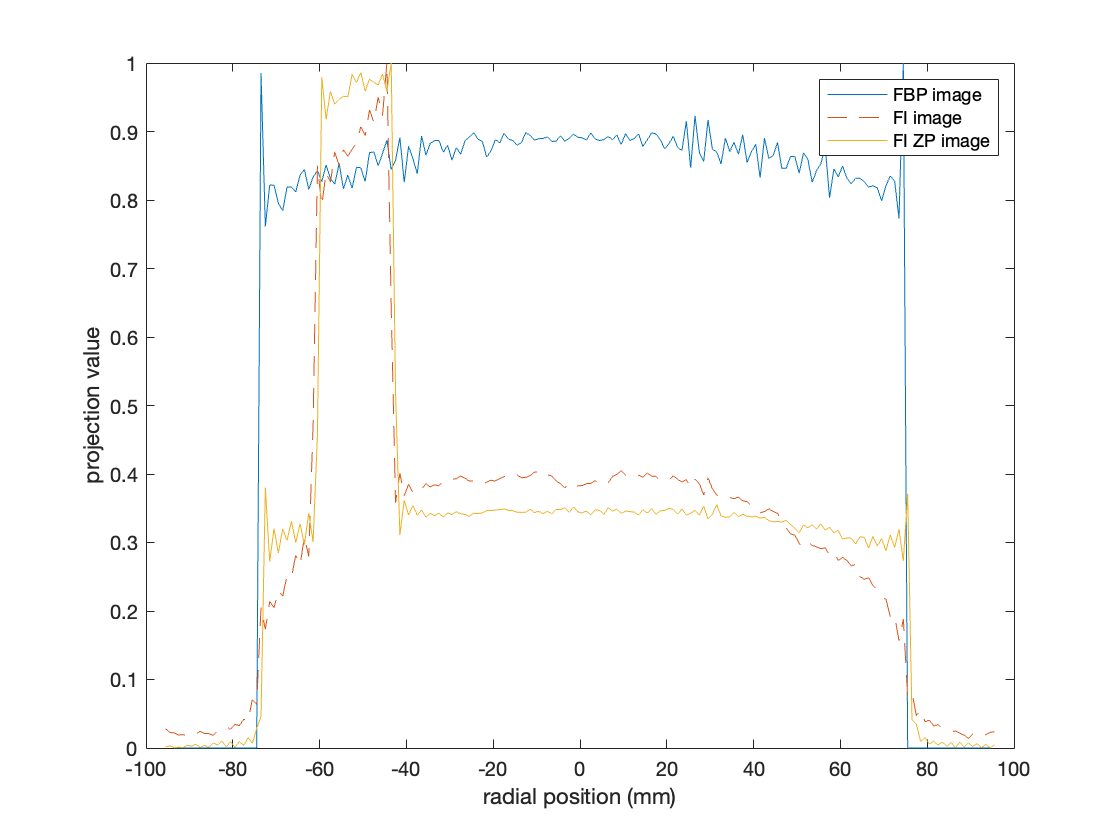
\includegraphics[width=1\textwidth]{8.png}
    \caption{Compared the signals based on different method.}
\end{figure}
\newpage 
%page 9
\section[short]{PART 9}
1. \textbf{FBP Reconstruction with Subsampling (Left Image)}: This image appears to have streak 
artifacts. Streaks arise due to the incomplete projection information which causes 
inconsistencies in the backprojected image. The edges of the objects in the image 
also appear less sharp, which is an indication of reduced spatial resolution due to subsampling.\\

2. \textbf{FI Reconstruction with ZP and Subsampling (Right Image)}: The FI method 
with zero padding seems to mitigate some of the streaking seen in the FBP image. 
The edges of the objects appear smoother, which suggests that the interpolation 
and zero padding may help compensate for the lower sampling rate to some extent. 
However, there may still be a loss of detail, and the image could exhibit interpolation 
artifacts that manifest as blurring or distortions.\\

In summary, both image looks less detailed with more artifacts due to the subsampling,
but the image based on the FI mehod was shown better performance than FBP reconstruction.

\begin{figure}[hb]
    \centering
    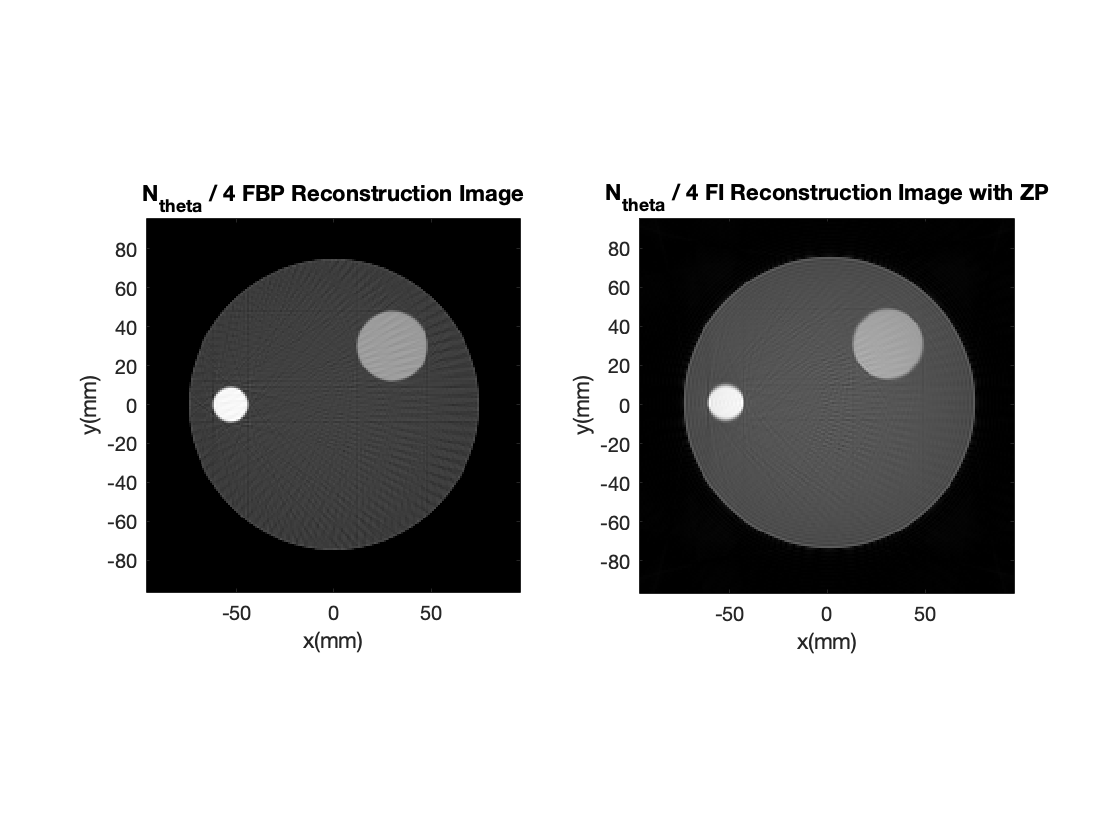
\includegraphics[width=1\textwidth]{9.png}
    \caption{$\frac{1}{4}$ subsampling.}
\end{figure}
\newpage 
%page 10
\section[short]{PART 10}
After the incomplete projections, the image looks far incorrect than the expected image
and the following artifacts could be detected:\\

1. \textbf{Streak Artifacts}: Due to the limited number of angles, streaking artifacts become
much more obvious. These appear as lines radiating from high-density areas to 
the rest of the image.\\

2. \textbf{Blurring}:The details in the image are likely to be less sharp 
because fewer projections mean less information to accurately reconstruct the image.\\

3. \textbf{Increased Noise}\\

In summary, From the provided image, we can observe a significant distortion and 
streaking, as expected. The limited projection data causes the reconstruction 
algorithm to inadequately represent the object, resulting in a loss of detail 
and the introduction of significant streaking artifacts. The boundaries between 
different structures within the image are also likely less defined, and there might 
be areas where the reconstruction has failed to represent the actual attenuation 
values correctly.
\begin{figure}[hb]
    \centering
    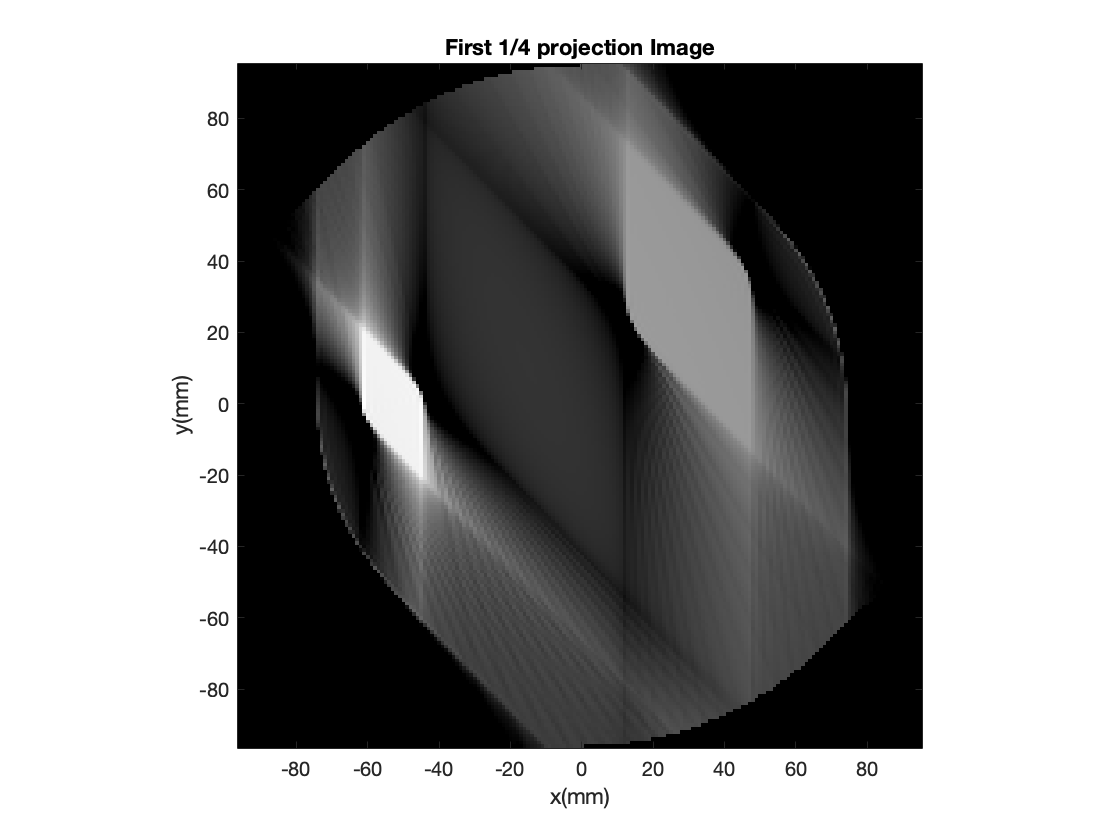
\includegraphics[width=0.75\textwidth]{10.png}
    \caption{$\frac{1}{4}$ subprojection.}
\end{figure}
\newpage 
%page 11
\section[short]{PART 11}
From the figure 11, we can find the image is "Minion" from the "Despicable Me" film series.\\

\begin{figure}[hb]
    \centering
    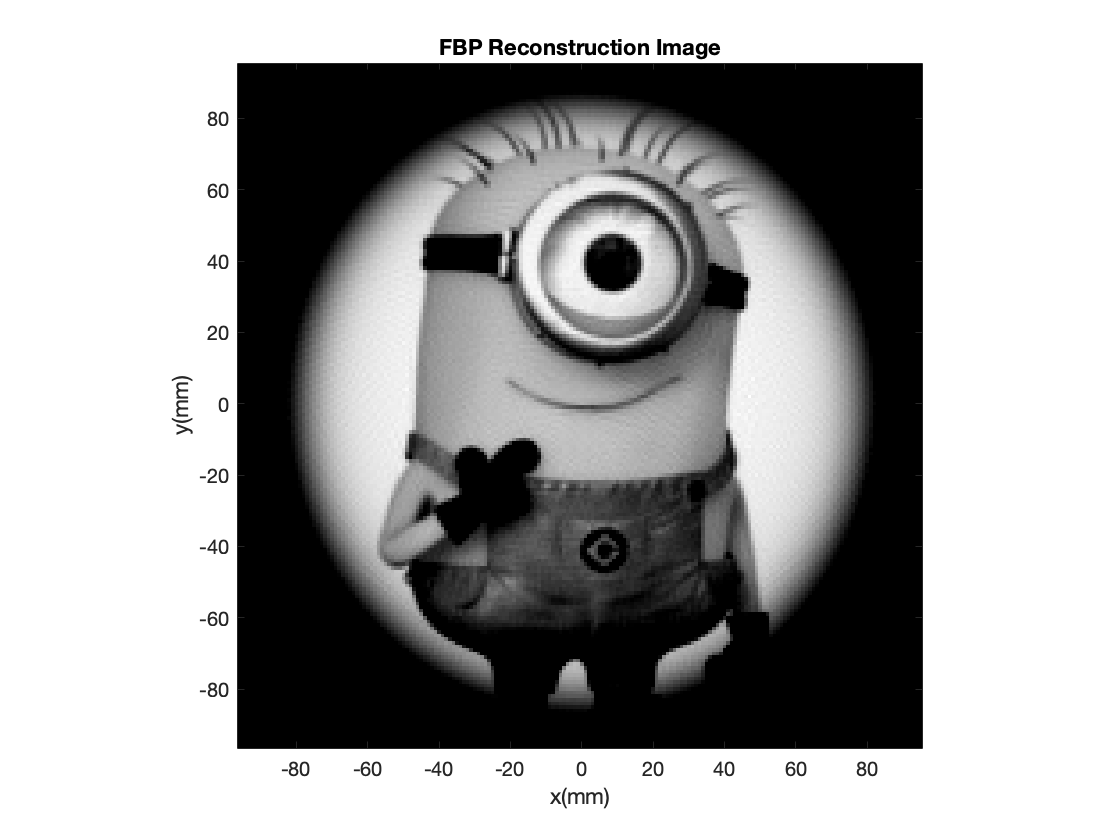
\includegraphics[width=1\textwidth]{11.png}
    \caption{Mystery Image.}
\end{figure}
\newpage 

From the Sinogram, it is really hard to guess the shape of image after deconstruction.
However, there are still some details could be noticed, such as the huge circle in 
$(R, \theta) = (0,\pi)$, the asymmetric hyperbolic curves starts approximately from 
$(R, \theta) = (10,0)$ and ends to $(R, \theta) = (10,2 \pi)$ seems like the boundaries
of the single eye and goggles.

\begin{figure}[hb]
    \centering
    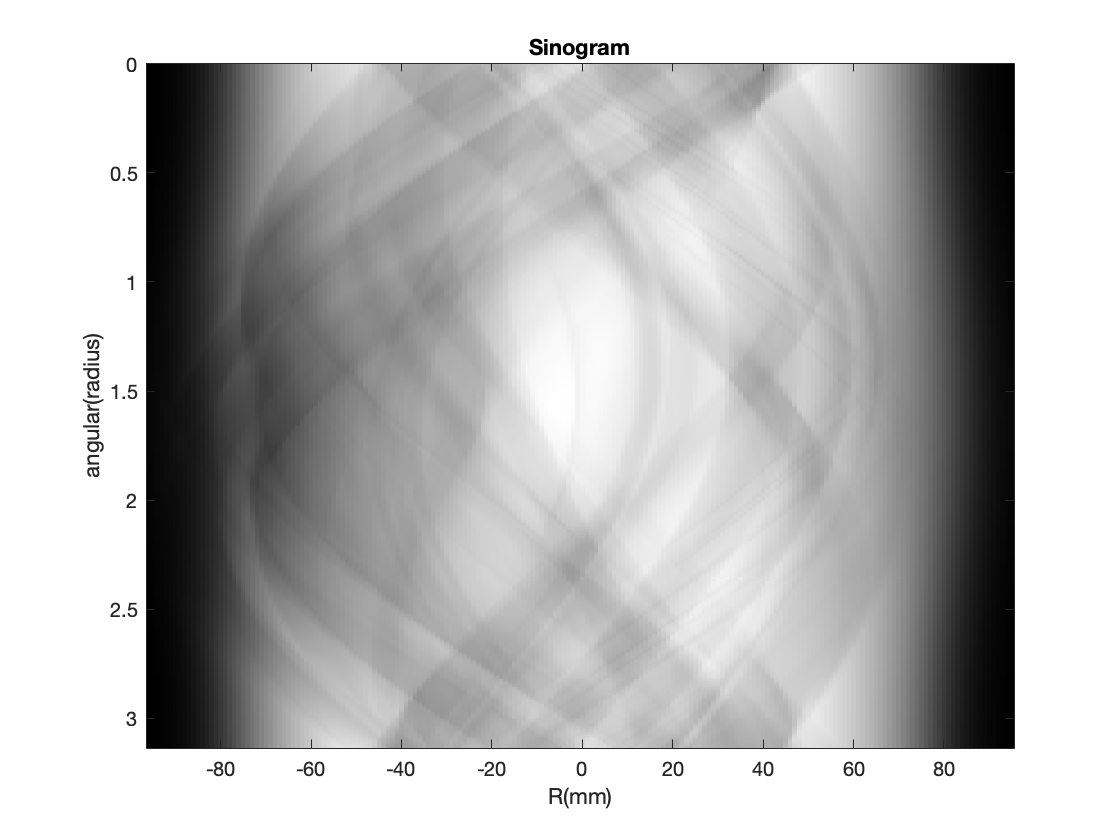
\includegraphics[width=1\textwidth]{12.png}
    \caption{Mystery Sinogram.}
\end{figure}
\end{document}